%%%%%%%%%%%%%%%%%%%%%%%%%%%%%%%%%%%%%%%%%%%%%%%%%%%%%%%%%%%%%%%%%%%%%%%%%%%%%%%%
% Preámbulo                                                                    %
%%%%%%%%%%%%%%%%%%%%%%%%%%%%%%%%%%%%%%%%%%%%%%%%%%%%%%%%%%%%%%%%%%%%%%%%%%%%%%%%

\documentclass[11pt,a4paper,titlepage,twoside,openright,openbib]{report}

%%% RELACIÓN DE VARIABLES A PERSONALIZAR %%%
%\def\lingua{gal}
\def\lingua{esp} % descomenta esta liña se redactarás a memoria en español
%\def\lingua{eng} % descomenta esta liña se redactarás a memoria en inglés
\def\nome{Alejandro Iregui Valcarcel}              % substitúe aquí o teu nome
\def\nomedirectorA{Outro Nome Completo}             % substitúe aquí o nome de quen dirixe
\def\titulo{eHand: control para prótesis mio-eléctrica de miembro superior} % substitúe aquí o título do teu TFG
%\def\mencion{NOME DA MENCIÓN}                        % descomenta a mención correspondente
%\def\mencion{COMPUTACIÓN}
%\def\mencion{ENXEÑARÍA DO SOFTWARE}
\def\mencion{ENXEÑARÍA DE COMPUTADORES}
%\def\mencion{SISTEMAS DE INFORMACIÓN}
%\def\mencion{TECNOLOXÍAS DA INFORMACIÓN}

\def\renomearcadros{si} % descomenta esta liña se redactas a memoria en español e prefires que
                         % os "cuadros" e o "índice de cuadros" se renomeen
                         % a "tablas" e "índice de tablas" respectivamente

\usepackage{estilo_tfg}

% Lista de paquetes potencialmente interesantes (uso baixo demanda)

% \usepackage{alltt}       % proporciona o entorno alltt, semellante a verbatim pero que respecta comandos
% \usepackage{enumitem}    % permite personalizar os entornos de lista
% \usepackage{eurofont}    % proporciona o comando \euro
% \usepackage{float}       % permite máis opcións para controlar obxectos flotantes (táboas, figuras)
% \usepackage{hhline}      % permie personalizar as liñas horizontais en arrays e táboas
% \usepackage{longtable}   % permite construir táboas que ocupan máis dunha páxina
% \usepackage{lscape}      % permite colocar partes do documento en orientación apaisada
% \usepackage{moreverb}    % permite personalizar o entorno verbatim
% \usepackage{multirow}    % permite crear celdas que ocupan varias filas da mesma táboa
% \usepackage{pdfpages}    % permite insertar ficheiros en PDF no documento
% \usepackage{rotating}    % permite diferentes tipos de rotacións para figuras e táboas
% \usepackage{subcaption}  % permite a inclusión de varias subfiguras nunha figura
% \usepackage{tabu}        % permite táboas flexibles
% \usepackage{tabularx}    % permite táboas con columnas de anchura determinada

%%%%%%%%%%%%%%%%%%%%%%%%%%%%%%%%%%%%%%%%%%%%%%%%%%%%%%%%%%%%%%%%%%%%%%%%%%%%%%%%
% Corpo                                                                        %
%%%%%%%%%%%%%%%%%%%%%%%%%%%%%%%%%%%%%%%%%%%%%%%%%%%%%%%%%%%%%%%%%%%%%%%%%%%%%%%%

\begin{document}

 %%%%%%%%%%%%%%%%%%%%%%%%%%%%%%%%%%%%%%%%
 % Preliminares do documento            %
 %%%%%%%%%%%%%%%%%%%%%%%%%%%%%%%%%%%%%%%%

 %\begin{titlepage}
  
  \hspace*{128pt}
  \textcolor{udcpink}{{\fontencoding{T1}\fontfamily{phv}\selectfont Facultade de Informática}}\\[-32pt]

  \begin{center}
    
\includegraphics[scale=0.3]{imaxes/udc}\\[35pt]

    {\large TRABALLO FIN DE GRAO \\
            GRAO EN ENXEÑARÍA INFORMÁTICA \\
            MENCIÓN EN \mencion } \\[100pt]
    
    \begin{huge}
      \begin{spacing}{1.3}
        \bfseries \titulo
      \end{spacing}
    \end{huge}
  \end{center}
  
  \vfill
  
  \begin{flushright}
    {\large
    \begin{tabular}{ll}
      {\bf Estudante:} & \nome \\
      {\bf Dirección:} & \nomedirectorA \\ % COPIA E PEGA ESTA LIÑA MÁIS VECES SE O PRECISAS
    \end{tabular}}
  \end{flushright}
  \rightline{A Coruña, \datasimple\today.}
\end{titlepage}

 %\paxinaenbranco
 %\dedicatoria{Dedicatoria} % escribe neste comando o teu texto de dedicatoria
 %\paxinaenbranco
 %\paxinaenbranco
 %\begin{agradecementos}
 %\blindtext   % substitúe este comando polo teu texto de agradecementos
 %\end{agradecementos}
 %\paxinaenbranco
 %%%%%%%%%%%%%%%%%%%%%%%%%%%%%%%%%%%%%%%%%%%%%%%%%%%%%%%%%%%%%%%%%%%%%%%%%%%%%%%%%

\begin{abstract}\thispagestyle{empty}
    En este documento se relata el proceso de creación que hay detrás de un controlador mio-eléctrico para una prótesis de miembro superior con amputación a nivel de mano.
    Dicho controlador leerá las señales \textit{EMG} que se producen en el paciente mediante electrodos colocados en el flexor carpi radialis y en el extensor carpi radialis longus,  músculos implicados en la pronación-supinación del antebrazo y flexo-extensión de la muñeca. Las señales serán filtradas por un controlador \textit{ARDUINO UNO} para finalmente ser procesadas por una red de neuronas primeramente simulada en Matlab y posteriormente implementada en \textit{FPGA}.
    % substitúe este comando polo resumo do teu TFG
    % na lingua principal do documento (tipicamente: galego)

  \vspace*{25pt}
  \begin{segundoresumo}
    This document describes the creation process behind a myoelectric controller for an upper limb prosthesis with hand-level amputation.
    The controller will read the \textit{EMG} signals that are produced in the patient by  electrodes placed on the flexor carpi radialis and on the extensor carpi radialis longus, muscles involved in pronation-supination of the forearm and flexion-extension of the wrist. 
    Signals are filtered by a microcontroller \textit{ARDUINO UNO} to finally be processed on a network of neurons first simulated in \textit{Matlab} and later implemented in \textit{FPGA}. 
    % substitúe este comando polo resumo do teu TFG
    % na lingua secundaria do documento (tipicamente: inglés)
  \end{segundoresumo}
\vspace*{25pt}
\begin{multicols}{2}
\begin{description}
\item [\palabraschaveprincipal:] \mbox{} \\[-20pt]
  \blindlist{itemize}[7] % substitúe este comando por un itemize
                         % que relacione as palabras chave
                         % que mellor identifiquen o teu TFG
                         % no idioma principal da memoria (tipicamente: galego)
\end{description}
\begin{description}
\item [\palabraschavesecundaria:] \mbox{} \\[-20pt]
  \blindlist{itemize}[7] % substitúe este comando por un itemize
                         % que relacione as palabras chave
                         % que mellor identifiquen o teu TFG
                         % no idioma secundario da memoria (tipicamente: inglés)
\end{description}
\end{multicols}

\end{abstract}

%%%%%%%%%%%%%%%%%%%%%%%%%%%%%%%%%%%%%%%%%%%%%%%%%%%%%%%%%%%%%%%%%%%%%%%%%%%%%%%%

 %\paxinaenbranco

 \pagenumbering{roman}
 \setcounter{page}{1}
 \bstctlcite{IEEEexample:BSTcontrol}

 \tableofcontents
 \listoffigures
 \listoftables
 \cleardoublepage
 
 \pagenumbering{arabic}
 \setcounter{page}{1}

 %%%%%%%%%%%%%%%%%%%%%%%%%%%%%%%%%%%%%%%%
 % Capítulos                            %
 %%%%%%%%%%%%%%%%%%%%%%%%%%%%%%%%%%%%%%%%

 %\chapter{Introdución}
\label{chap:introducion}

\lettrine{E}{l} uso de prótesis a falta de miembros en el cuerpo es una historia que nos persigue desde antes de Cristo, debido a las limitaciones de la época estamos hablando de implantaciones fijas sin ningún tipo de utilidad que lo largo de los años y con ayuda de los avances en electrónica y mecánica el ser humano ha sido capaz de mejorar. Actualmente, existen prótesis avanzadas que son capaces de devolver al paciente una importante variedad de movimientos. Aun así, debido a factores como el mercado de producción o la tecnología nos encontramos con productos que no están a la disposición de cualquiera, la relación precio/utilidad está muy presente en la vida de los amputados.\\

En cuanto a la facilidad que hay para acceder a herramientas de desarrollo en este tipo de proyectos en concreto, ya sean, elementos Hardware de sensorización, conversión analógico digital y Software especializado, fue difícil encontrar una plataforma con la que poder trabajar fácilmente y por poco precio. Este TFG tiene también como objetivo ayudar a identificar las mejores opciones y ofrecer herramientas de tipo Open Source que se puedan utilizar por cualquiera.\\

Para llegar a conseguir que las prótesis electromecánicas sean asequibles y llamativas de convertirse en un producto es interesante también analizar otros usos que se le puede dar y se le está dando a esta tecnología. Entre más utilizada sea, mayor mercado se creará, menores serán los costes, mejor será la competencia y en definitiva los productos verán aumentada su calidad. 
Este análisis de mercado se basará entonces en el concepto de que con la electromiografía, buscamos extraer información de la actividad actividad muscular para con ella reconocer patrones de movimientos e incluso extraer características de cada músculo implicado, por esto mismo descubrí que actualmente se empieza a ver aplicada en la fisioterapia como herramienta para la valoración muscular y del ejercicio en clientes.
La empresa española MDURANCE se encarga de suministrar este tipo de equipamiento para clínicas y ha conseguido una buena recepción entre sus compradores, ofreciendo tanto Hardware como Software listo para usar por los fisioterapeutas en sus sesiones.

\begin{figure}[hp!]
\begin{center}
    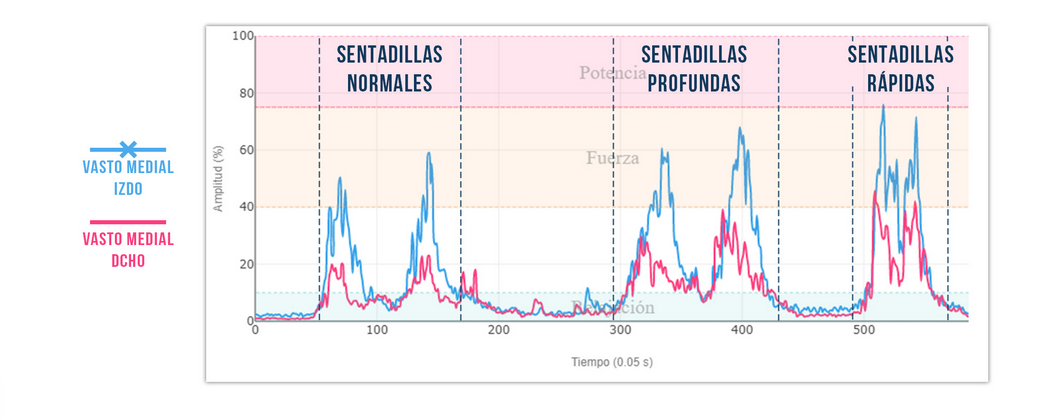
\includegraphics[width=1\textwidth]{imaxes/mdurance1.png}
    \caption{ActionButton}
    
    \vspace{1cm}

    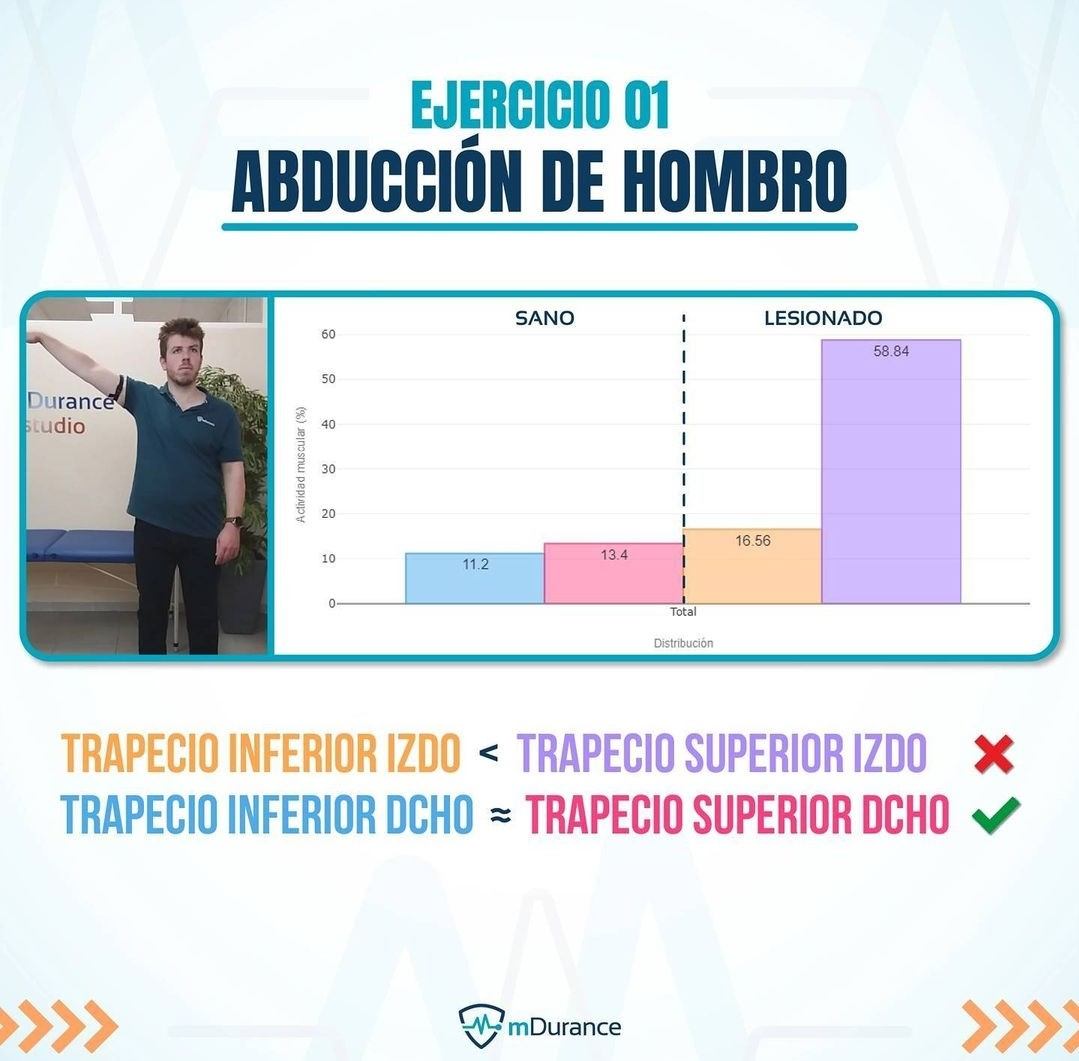
\includegraphics[width=0.75\textwidth]{imaxes/mdurance2.jpg}
   \vspace{0.1cm}
    \caption{ActionButton}
    \label{ActionButton}
  \end{center}
\end{figure}



Como se puede ver, este tipo de herramienta es utilizada para obtener lecturas de la actividad muscular durante ciertos movimientos y así ofrecer al especialista información más detallada e individual sobre sinergias musculares, descompensaciones, fatiga... 
Lo que más me parece interesante sobre el producto que ofrecen en MDURANCE es la escalabidad que tiene para implementar un sistema que no solo se base en la electromiográfia y pueda crecer hacia un asistente clínico que tenga capacidad de sacar conclusiones en base a diferentes datos que recolecta durante las sesiones. Ahora mismo, cuentan también con videofeedback y monitorización del progreso. 

Otro uso interesante que se podría ver en el mercado de la electromiografía se encuentra en las interfaces hombre-máquina, donde se podría utilizar como método para controlar elementos externos mediante la caracterización de movimientos. Un ejemplo sencillo se encontraría dentro de la Realidad Virtual, en donde se busca sumergir a la persona en un mundo completamente digital, donde existe un avatar controlado por los movimientos de la misma. Y no solo eso, los juegos también son un método interesante para introducir a la gente en este tipo de tecnologías y hacer más amigable la interacción durante los experimentos para así, enseñar de forma gráfica y divertida de que se trata. A parte de esto, también se puede pensar en utilizarlo para controlar cualquier tipo de máquina.\\

\begin{figure}[!h]
  \centering
  \begin{tabular}[c]{cc}
    \begin{subfigure}[c]{0.5\textwidth}
      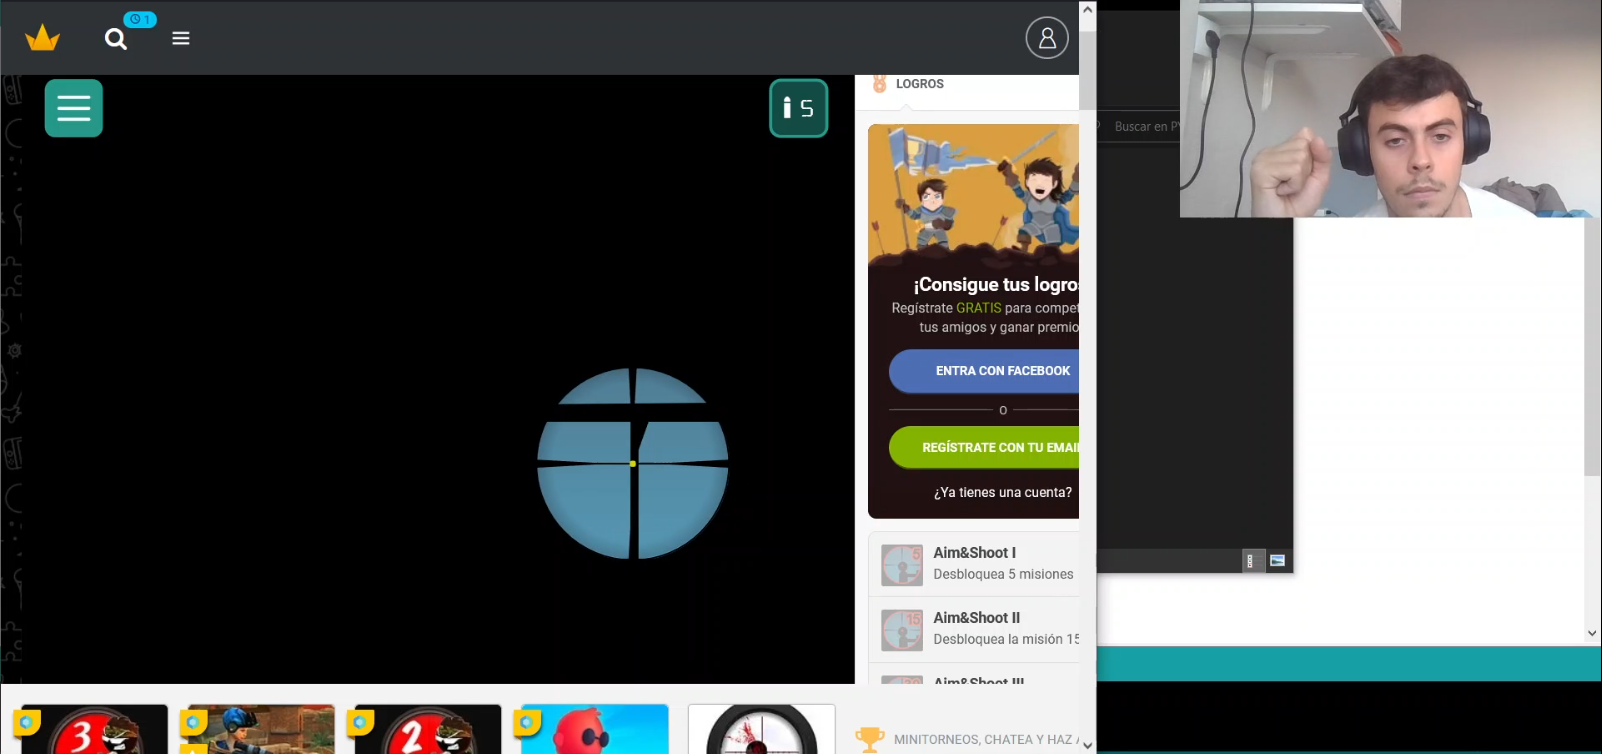
\includegraphics[width=\textwidth]{imaxes/juego1.png}
      
    \end{subfigure}&
    \begin{subfigure}[c]{0.5\textwidth}
      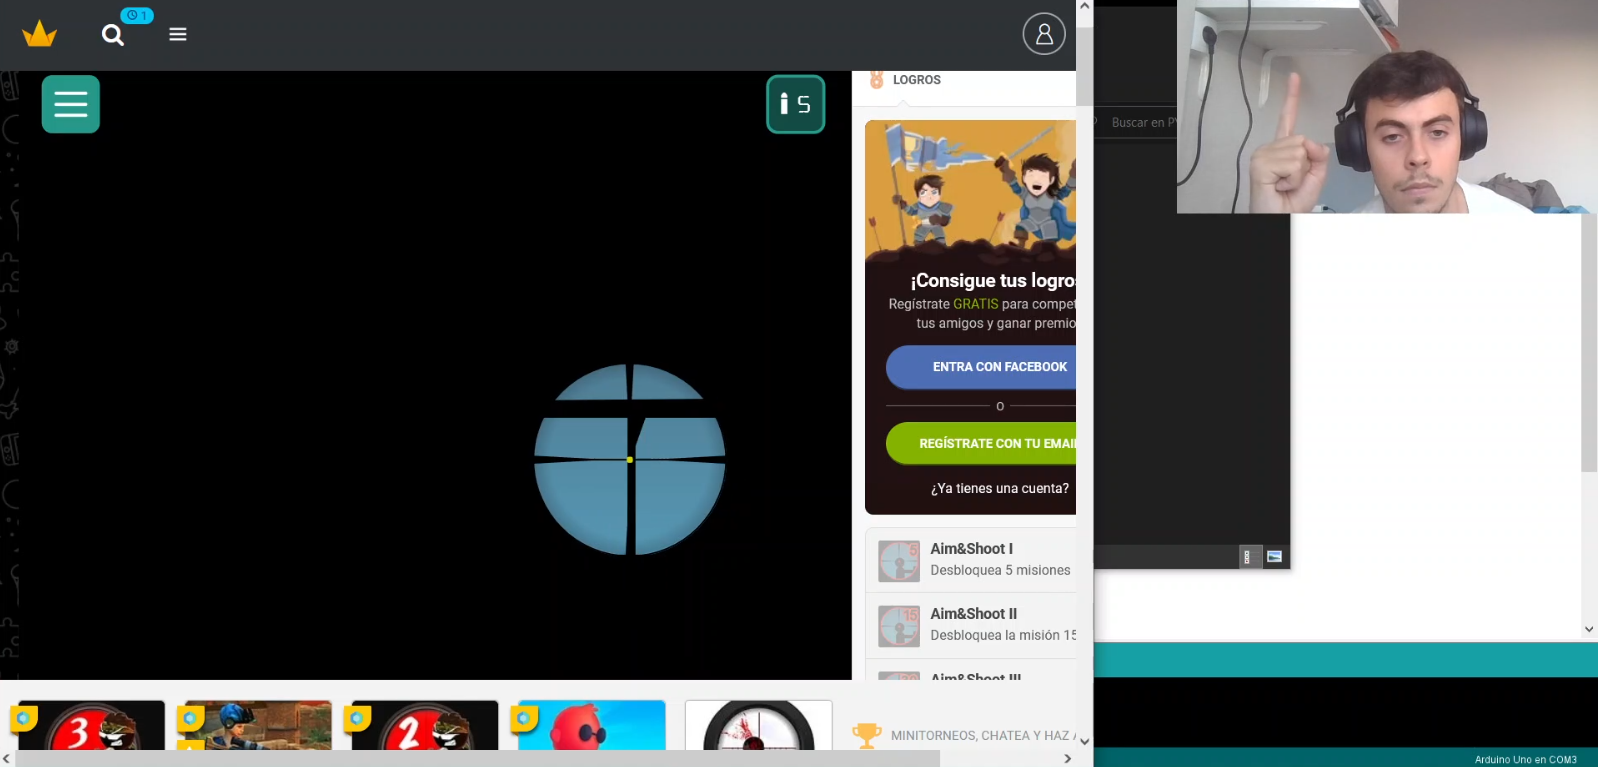
\includegraphics[width=\textwidth]{imaxes/juego2.png}
      
      
    \end{subfigure}\\
    \begin{subfigure}[c]{0.5\textwidth}
      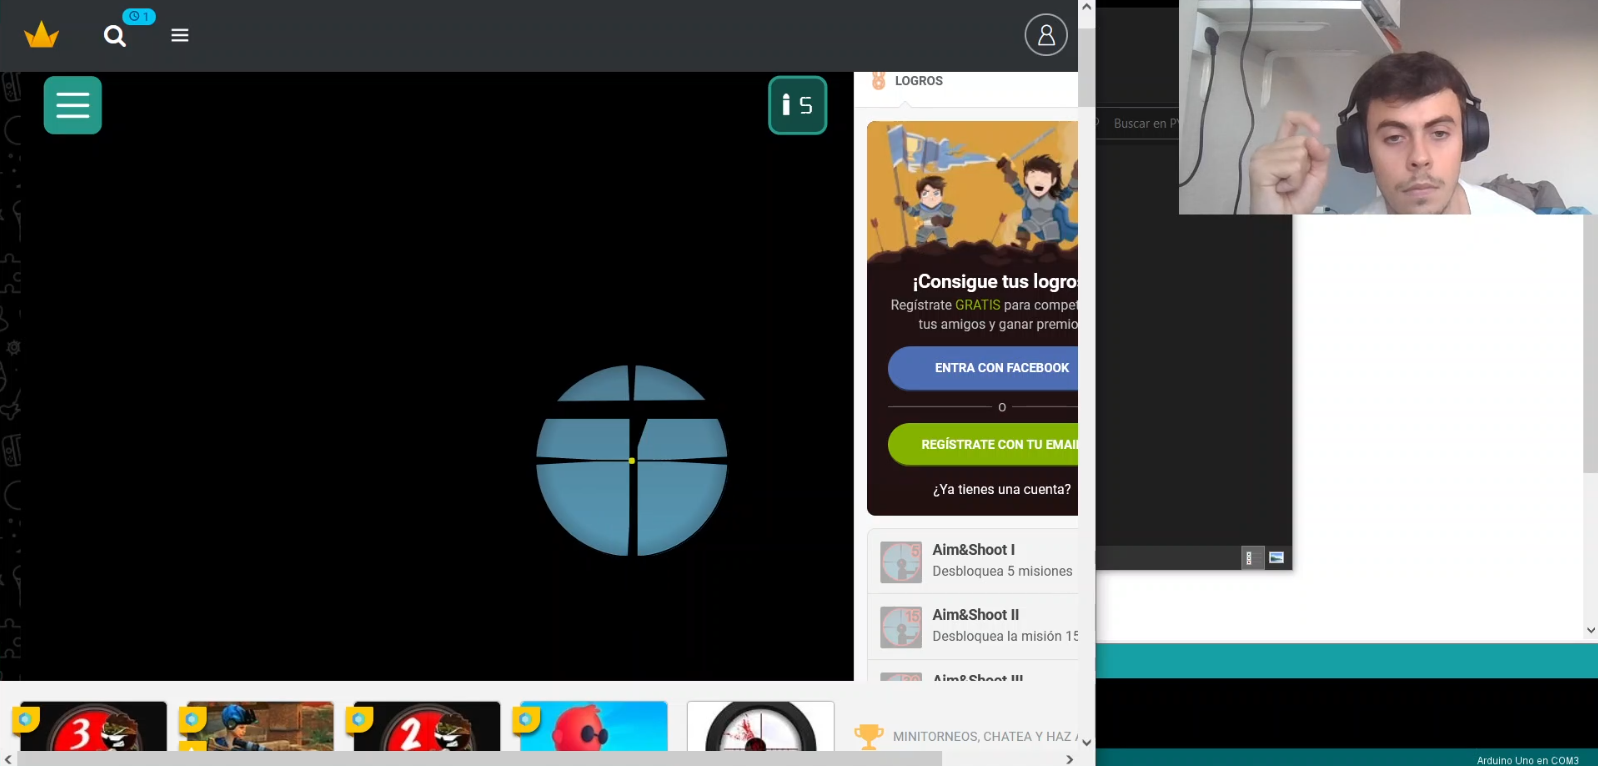
\includegraphics[width=\textwidth]{imaxes/juego3.png}
      
    \end{subfigure}&
    \begin{subfigure}[c]{0.5\textwidth}
      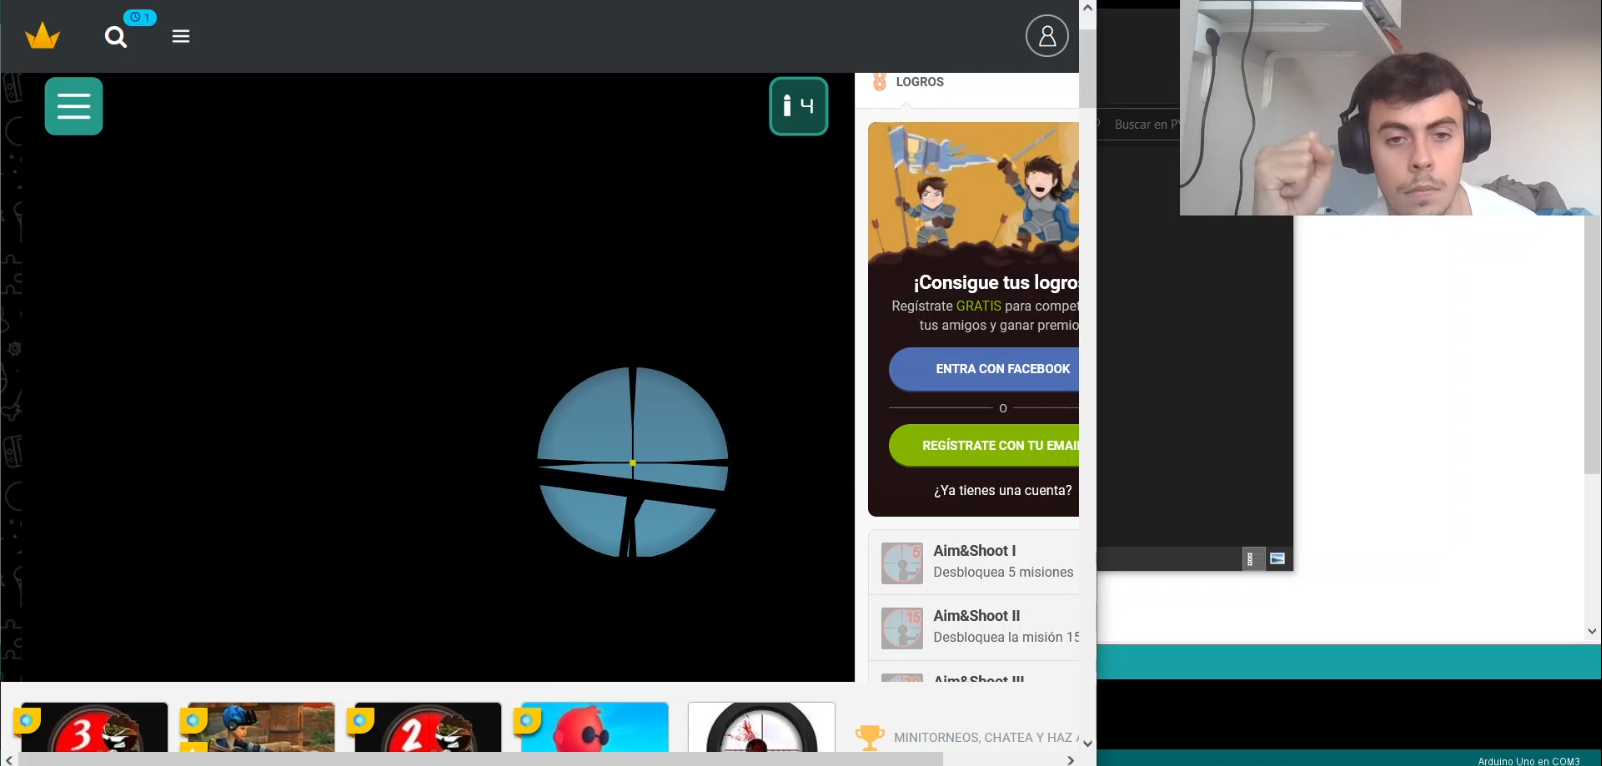
\includegraphics[width=\textwidth]{imaxes/juego4.png}
      
    \end{subfigure}\\
  \end{tabular}    
 
\end{figure}


\section{Anatomía básica y lectura de señales}
\label{sec:mostra}

Los músculos son un tipo de tejido blando que puede contraerse mediante impulsos nerviosos, generando movimiento y permitiendo trabajos mecánicos. La electromiografía es una técnica que mide la actividad eléctrica generada por el paso del impulso nervioso, que provoca la despolarización de la membrana de la célula muscular durante la excitación. Si la despolarización alcanza un determinado valor umbral, se genera un potencial de acción.\\

\begin{figure}[hp!]
\begin{center}
    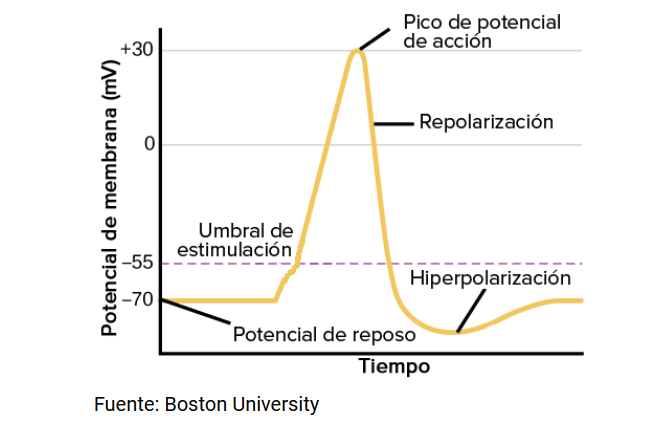
\includegraphics[width=1\textwidth]{imaxes/emg.png}
    \caption{ActionButton}
    
    \vspace{1cm}

    \label{ActionButton}
  \end{center}
\end{figure}


Para las mediciones, comúnmente se hace uso de dos emisores (uno en cada extremo del musculo a medir) y un GND (normalmente ubicado en zona de hueso) para extraer una señal mas limpia que posteriormente se amplifica y filtra. Son también llamamos electrodos y existen diferentes tipos de los mismos en los que podemos diferenciar los pasivos, activos, húmedos o en seco. Sobre ellos creo que actualmente los más cómodos de utilizar los secos, ya que permiten una fácil interacción y se pueden recolocar facilmente, igualmente pienso en que habría que reinventar un poco el formato en el que se utilizan.

Por tanto, la EMG mide de una manera indirecta la actividad muscular, ya que es capaz de determinar si el sistema nervioso está reclutando activamente un músculo durante una tarea específica.(MDURANCE)\\

Aplicado al control de prótesis es importante reconocer y estudiar las zonas de donde se van a tomar las lecturas, dependerá del tipo de amputación, del numero de señales que queramos usar para el control e incluso de características como el porcentaje de grasa que tiene el paciente en cuerpo, la edad.. En nuestro caso al tratarse de una prótesis de 2 canales mediremos la actividad del flexor carpi radialis y el extensor carpi radialis longus. Estos músculos ubicados en el antebrazo están implicados en varios movimientos de la mano, el flexor carpi tiene la acción de flexor principal de la muñeca, con tendencia a su abducción y pronación. También es flexor del codo. El otro, en la articulación del codo realiza ligera flexión y en la de la muñeca extensión colaborando en el cierre del puño y desviación radial.\\ 

De esta zona podríamos diferenciar señales incluso provenientes de cada dedo por individual, pero ello implicaría mayor y mejor sensorización y una capacidad de inteligencia superior en el controlador para diferenciar las señales provenientes de cada movimiento, esto sería lo mas interesante si queremos imitar al máximo el comportamiento de una mano pero tendría ciertas restricciones como el aumento del costo, un periodo mayor de adaptación y entrenamiento para el paciente e incluso un incremento en el tamaño o en el peso de la implantación. Lo que busco en este proyecto, es desarrollar un sistema funcional al precio mas bajo que sea capaz de conseguir, adelantando ya que es posible conseguir muy buenos resultados a bajo coste.

\begin{figure}[hp!]
\begin{center}
    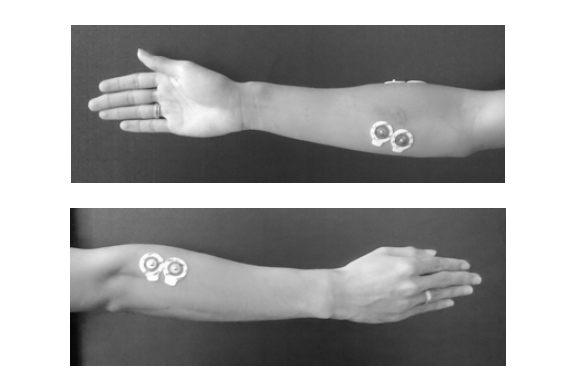
\includegraphics[width=0.75\textwidth]{imaxes/electrodos.png}
    \caption{ActionButton}
    
    \vspace{1cm}

    \label{ActionButton}
  \end{center}
\end{figure}



%\subsection{Subsección de mostra}
%\Blindtext

 \chapter{Placas, configuración para las lecturas y primeras muestras}
\label{chap:cap1}

\lettrine Cual sería entonces la forma de leer estas señales de forma fácil? Esta fue la pregunta que me hice y mi primer recurso de información para responderla fue internet. Indagando encontré que existían algunos fabricantes estadounidenses de PCBs para desarrollo que ofrecían soluciones de difícil acceso y a coste alto. Por ello seguí buscando y topé con un canal llamado "Biomakers" en donde había tutoriales muy buenos sobre EMG, ECG, EEG, e incluso, enseñaba diseños para la circuitería necesaria. Quiero comenzar este capítulo entonces hablando a grandes rasgos de la composición de los mismos ya que me sorprendió lo sencillos que son. El principio básico de un sensor se trata en mapear una magnitud real como la luz, la temperatura u otros en funciones matemáticas, extraemos valores del mundo que nos rodea para poder representarlos de forma transductible. En este caso al estar leyendo los pocos milivoltios que se generan durante la actividad muscular, entre nuestra señal y sensor no existirá la necesidad de hacer transformaciones entre magnitudes ya que simplemente servirá como amplificador de la actividad para obtener un señal manipulable.

\begin{figure}[hp!]
\begin{center}
    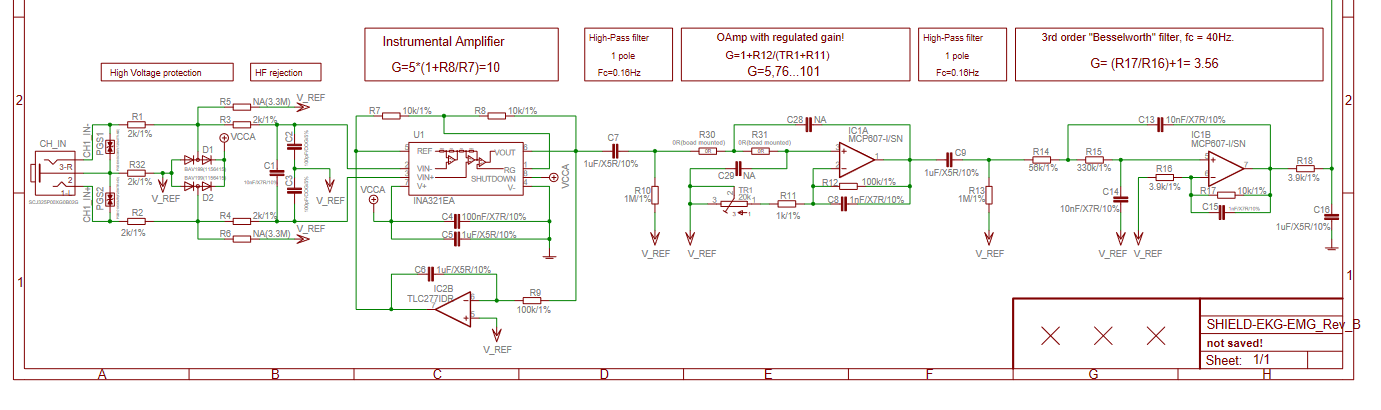
\includegraphics[width=0.95\textwidth,scale=0.5, height=5.5cm]{imaxes/circuito.png}

  \end{center}
\end{figure}

El circuito de la figura hace referencia a la placa SHIELD-EKG-EMG de Olimex, como su nombre indica se trata de un "escudo" que se puede apilar sobre las placas de tipo Arduino Uno y cuenta con todos los componentes para ser calibrada y conectada a la misma. Esta parte de su esquemático se corresponde con la del sensor electromiográfico. 

Empezando desde las izquierda del todo vemos que existe una conexión "CH\_IN" en donde tenemos 3 terminales de conexión L, R y Masa, correspondiéndose cada uno con los terminales de los 3 electrodos. A grandes rasgos, lo que podemos ver es que las corrientes recogidas por estos elementos irán pasando por varias fases de amplificación y filtrado. Comenzando por componentes de protección pasamos a una etapa en donde rechazaremos frecuencias altas y a continuación, amplificaremos la señal mediante un Amplificador Operacional de cierta ganancia. Seguimos entonces con etapas de filtrado para la frecuencia de 0 Hz característica de la corriente continua para finalmente, llegar a una etapa que creo merece cierta explicación.

En este caso se trata de una fase en donde utilizaremos un Amplificador de ganancia regulada. Y porque regulada? Bien, durante la introducción explicaba que este tipo de sensores va a estar afectado por ciertas características físicas de la persona y puede ocurrir, que no tenga la sensibilidad suficiente para recoger señales desde la superficie (ya sea por el índice de grasa que separa el sensor y el músculo o también por la poca masa muscular de la zona). Por esto mismo la PCB de Olimex nos permite adaptarnos a cualquier situación. La calibración para esta placa en mi opinión es un poco engorrosa ya que se hace de forma física y mediante una señal PWM que genera, por lo que sería interesante que se pudiese hacer de manera completamente Software.

Pasando a la configuración de sensores y microcontroladores que se utilizó para este proyecto, el sensor de Olimex no fue el único componente que utilicé para los experimentos y en realidad, los resultados que figurarán aquí se corresponden con otra placa. Esto también merece explicación ya que antes de descubrir la antes descrita, un día tuve la suerte de toparme con la siguiente PCB de China.

\begin{figure}[hp!]
\begin{center}
    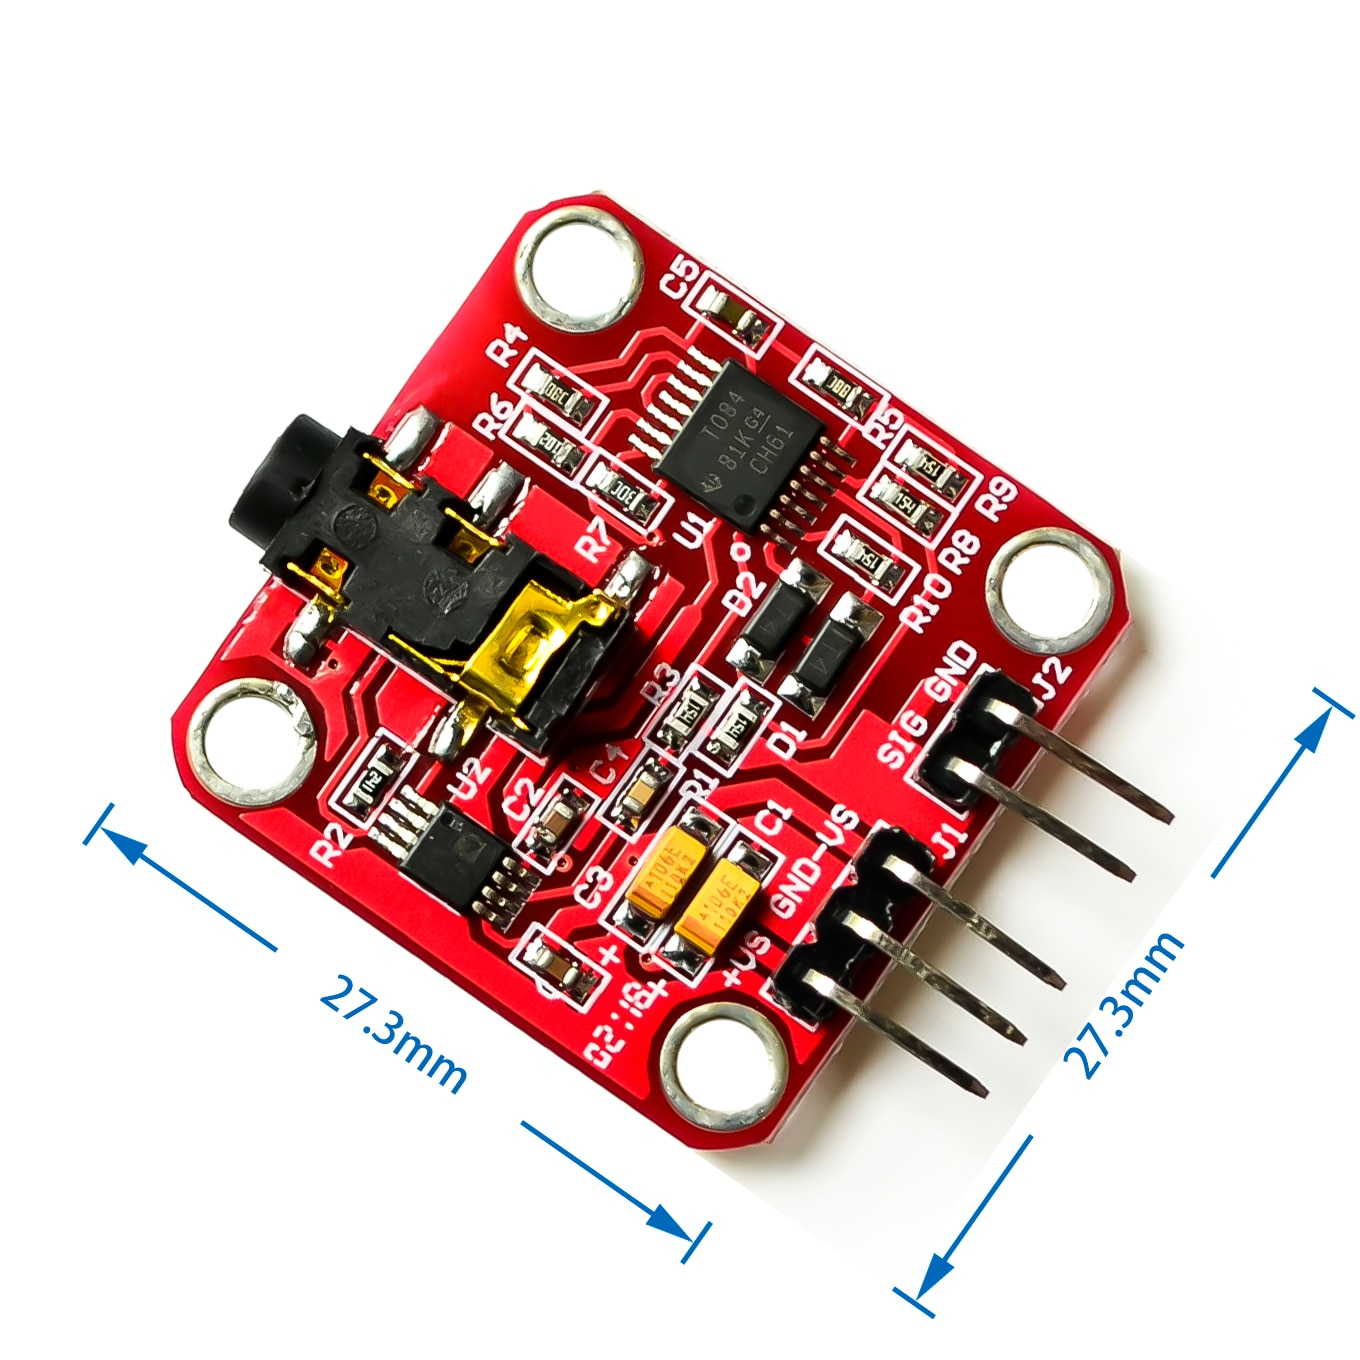
\includegraphics[width=0.6\textwidth, height=5cm]{imaxes/placa_china.jpg}
    \caption{ActionButton}
    \label{fig:plot}
  \end{center}
\end{figure}

Concretamente la encontré en Aliexpress y por 15€, trae un pack con los electrodos, parches y sensor. Desde que me llegó y la probé me di cuenta de que era la indicada para este proyecto, el precio es irresistible, el tamaño y la utilidad que ofrece es muy buena, además, es muy fácil de poner a funcionar. Para ello necesita una alimentación de +9v y -9v, utiliza la referencia positiva y negativa para hacer operaciones, la salida la da por el terminal de "sig" y se trata de una señal analógica de entre 0v y 3v, es decir, completamente positiva (esto tiene sentido porque el Arduino es incapaz de leer voltajes negativos en sus terminales analógicos).    
\vspace{0.15cm}

Por lo tanto contamos con el siguiente Setup para los experimentos:
\begin{itemize}
  \item 2 Placas PCB.
  \item Arduino UNO.
  \item Electrodos en seco y húmedos.
\end{itemize}

\begin{figure}[hp!]
\begin{center}
    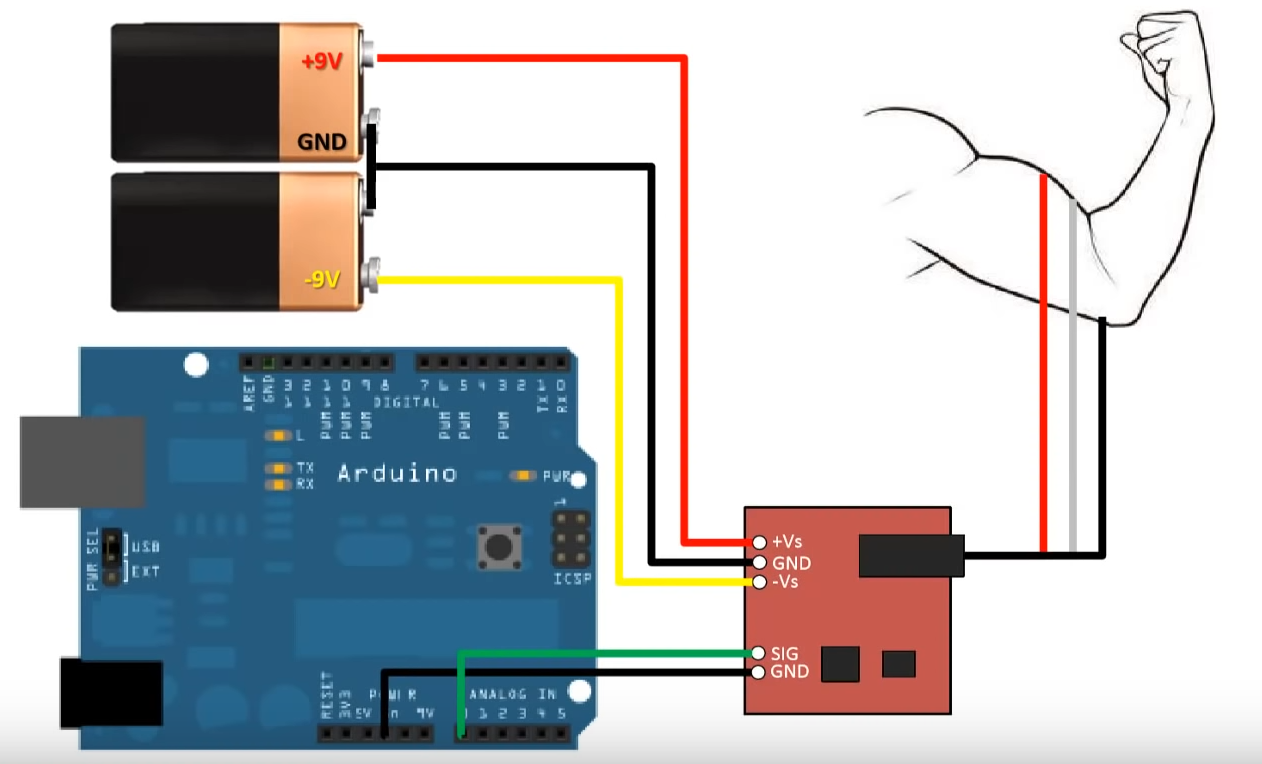
\includegraphics[width=100mm, height=5cm, scale=0.5]{imaxes/montaje.png}
    
    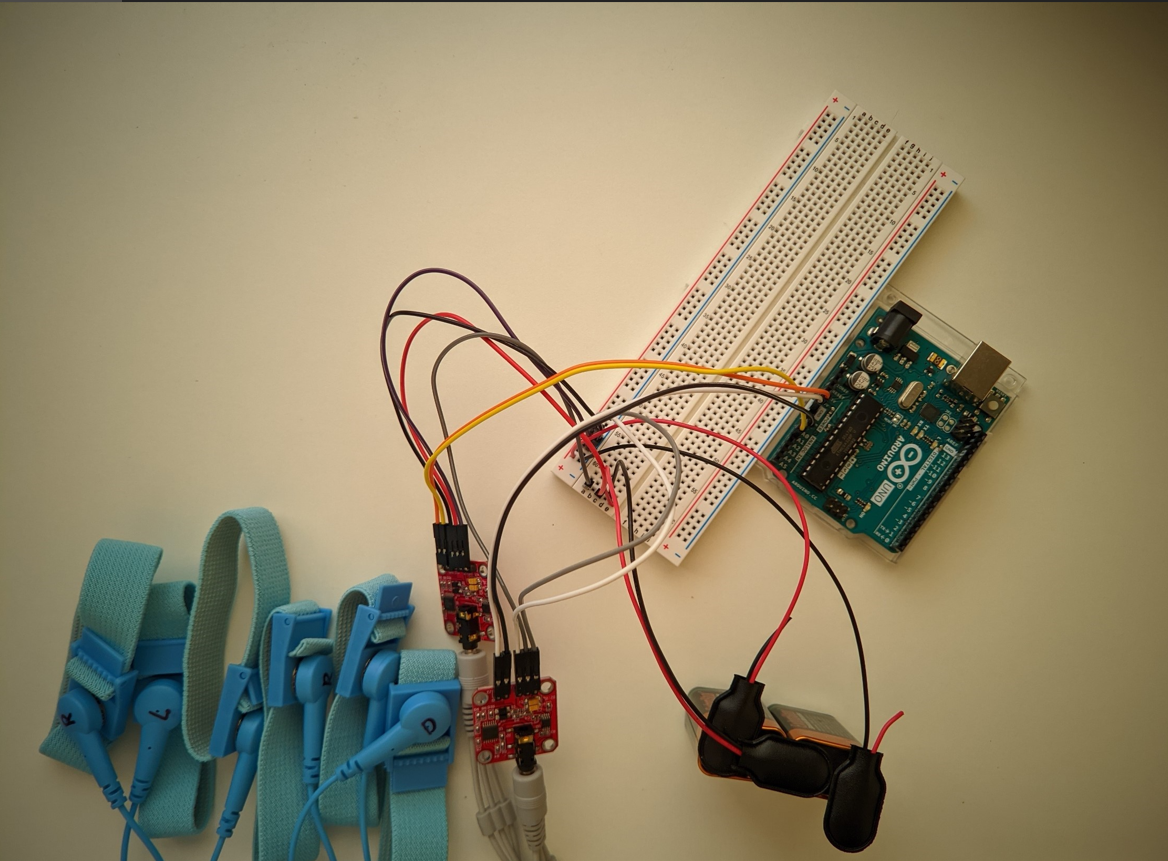
\includegraphics[width=12.5cm, height=6.5cm, scale=0.5]{imaxes/configuracion.png}
    \caption{ActionButton}
    \label{ActionButton}
  \end{center}
\end{figure}

El montaje es bastante trivial, lo puede hacer cualquiera en casa y con un kit de principiantes para electrónica. Se puede ver que que con 10 cables estaría todo montado, por lo que sería muy fácil con este tamaño e incluso un Arduino del tipo Nano diseñar una carcasa a impresora 3d, para acoplarlo todo de forma cómoda.

Después de habernos colocado los electrodos, comenzar a leer los primeros valores es tan fácil como configurar en el código del Arduino el puerto serial y leer dentro del loop por los puertos Analógicos. Aclarando ahora que no voy a entrar en detalles sobre el código ya que es muy simple el funcionamiento y todo estará completamente disponible in mi GitHub.\\ 

\begin{figure}[hp!]
\begin{center}
    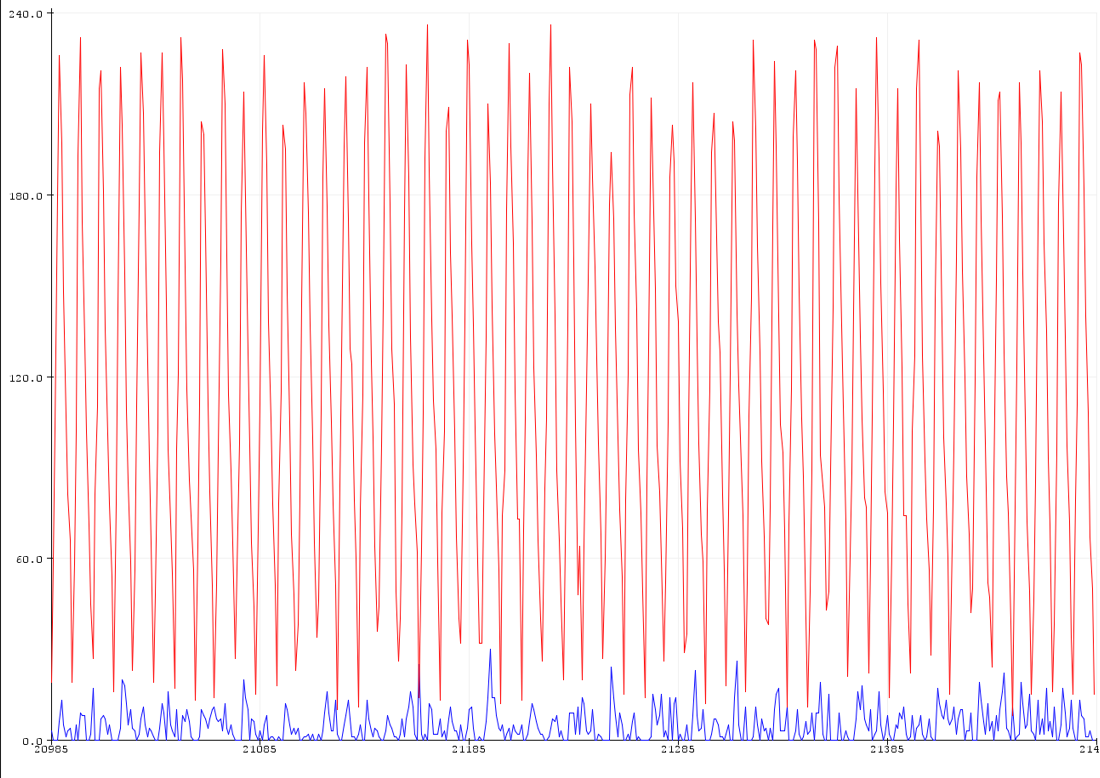
\includegraphics[width=0.75\textwidth, scale=0.5]{imaxes/resting.png}
    \caption{ActionButton}
    \label{fig:plot}
  \end{center}
\end{figure}

La figura \autoref{fig:plot} se trata de un ejemplo de dibujo para las 2 señales de nuestros músculos en reposo, se trata de un plot en tiempo real que nos muestra la herramienta de Serial Plotter y que trae el IDE de Arduino.

Para todos los experimentos configuramos una frecuencia de muestreo a 1000 Hz y BaudRate de 115200. El porqué del primer parámetro se basa en las siguientes 2 ideas:

\begin{itemize}
  \item Las frecuencias significativas en el EMG se encuentran entre los 0Hz y los 500Hz, siendo esta última una opción también para configurar y evitar Aliasing. 
  \item Si se quieren buenos resultados en la prótesis, la respuesta como aplicación de ingeniería debe ser menor a los 300ms, por lo que haciendo cálculos unas 250 muestras serían suficientes para extraer patrones. 
\end{itemize}

Añadir que aunque buscamos buenos resultados con 250 muestras, es recomendable en las mediciones capturar muchas más para tener de sobra durante los análisis.\\ 
Para las mediciones finales, se creó una herramienta Software en Python que se encarga de conectarse al Arduino, sincronizarse con él, leer las muestras de los 2 canales y exportarlas a CSV. A parte de estos comportamientos, también ofrece un menú simple por comandos en el que se puede gestionar el tipo de medición que estamos haciendo, llevar la cuenta de las mismas, plottear el resultado e incluso interaccionar con el usuario mediante un sonido para indicarle cuando debe realizar el movimiento.

Una vez tenemos todo configurado podemos pasar a relizar las primeras mediciones, empezaremos entonces con los siguientes 3 estados:

\begin{itemize}
  \item Flexión de muñeca. 
  \item Extensión de muñeca.
  \item Reposo.
\end{itemize}

\begin{figure}[!h]
  \centering
  \begin{tabular}[c]{cc}
    \begin{subfigure}[c]{0.5\textwidth, scale=0.5}
      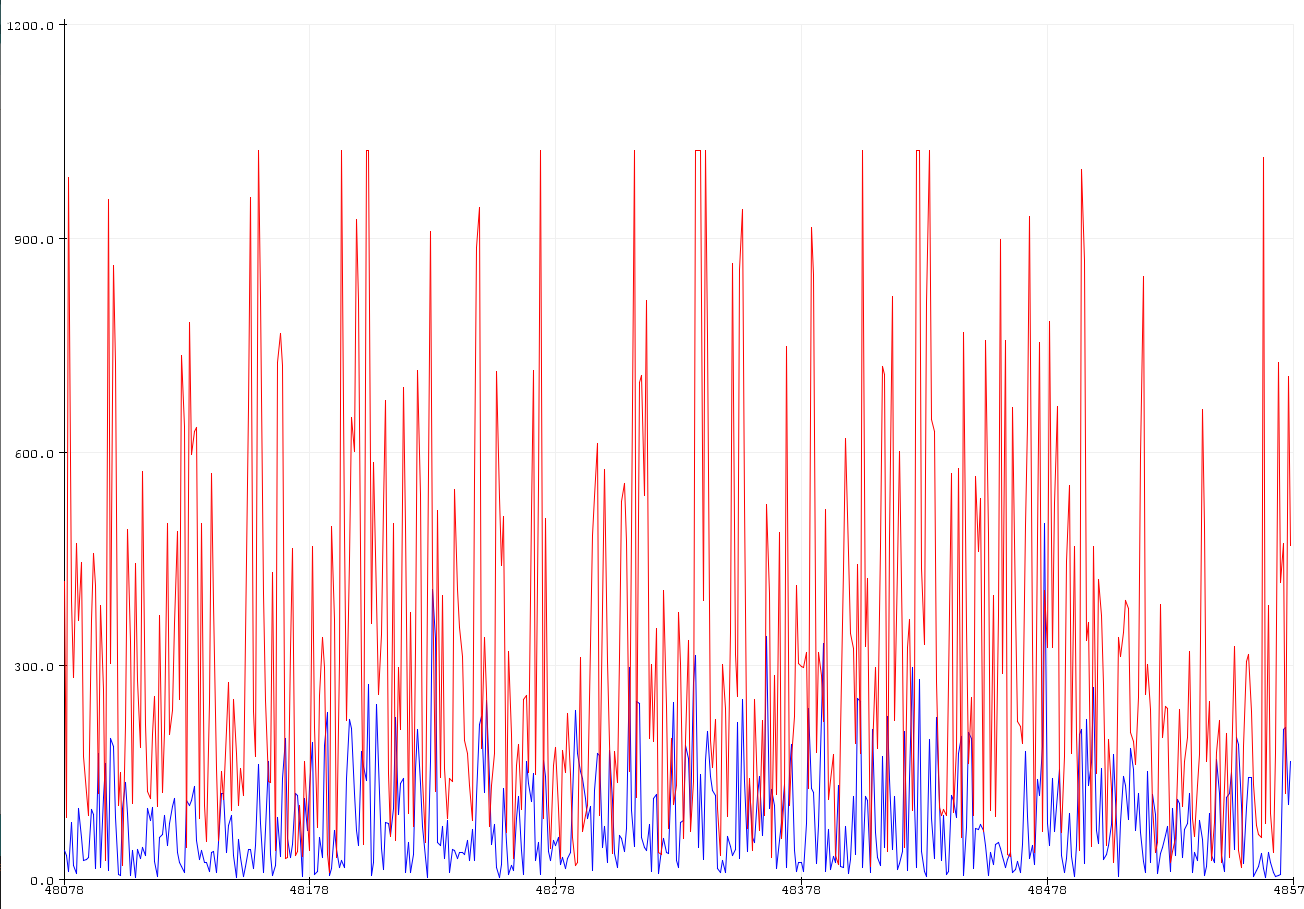
\includegraphics[width=\textwidth]{imaxes/flexion.png}
      
    \end{subfigure}&
    \begin{subfigure}[c]{0.5\textwidth, scale=0.5}
      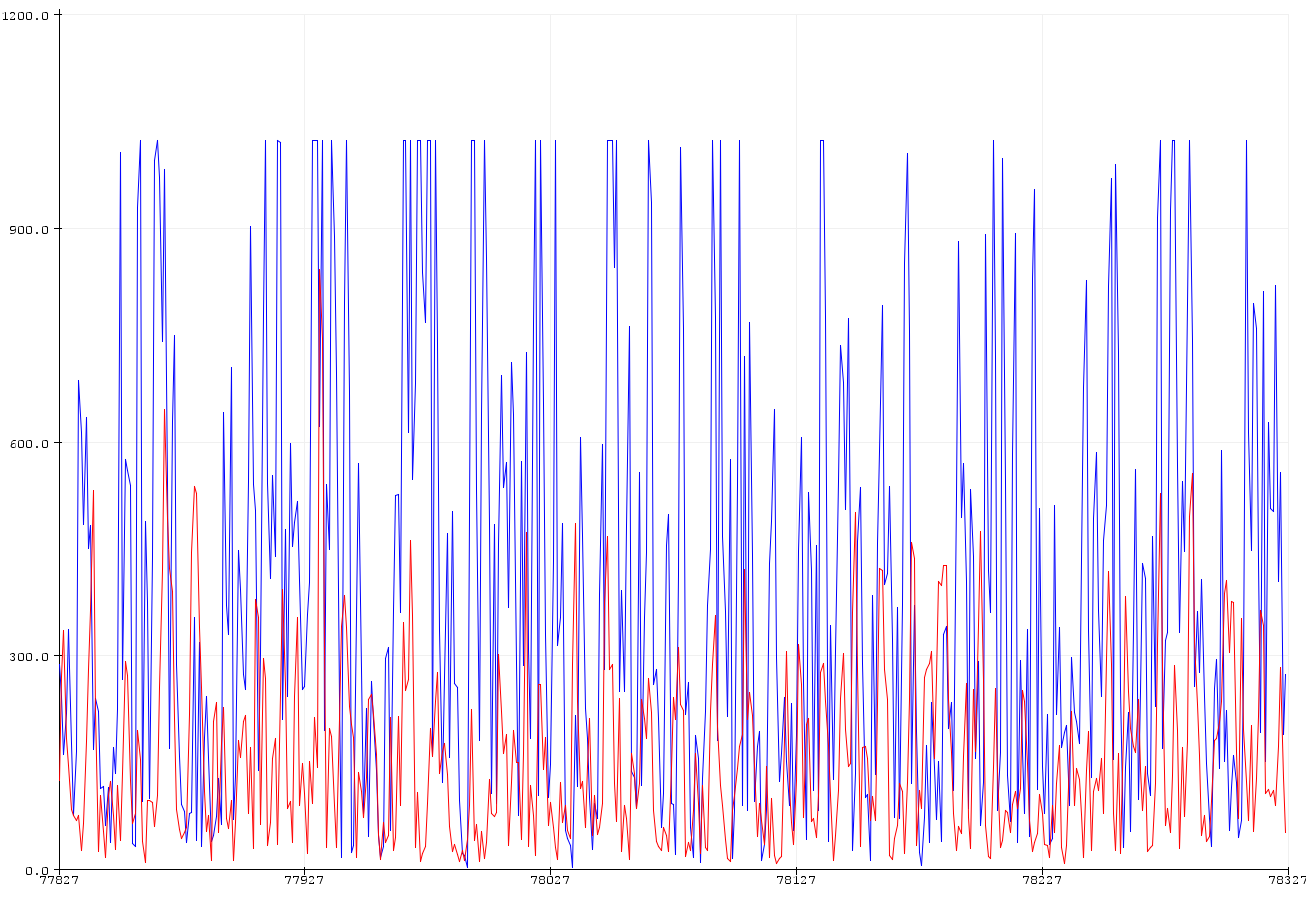
\includegraphics[width=\textwidth]{imaxes/extension.png}
      
    \end{subfigure}&
    \begin{subfigure}[c]{0.5\textwidth, scale=0.5}
      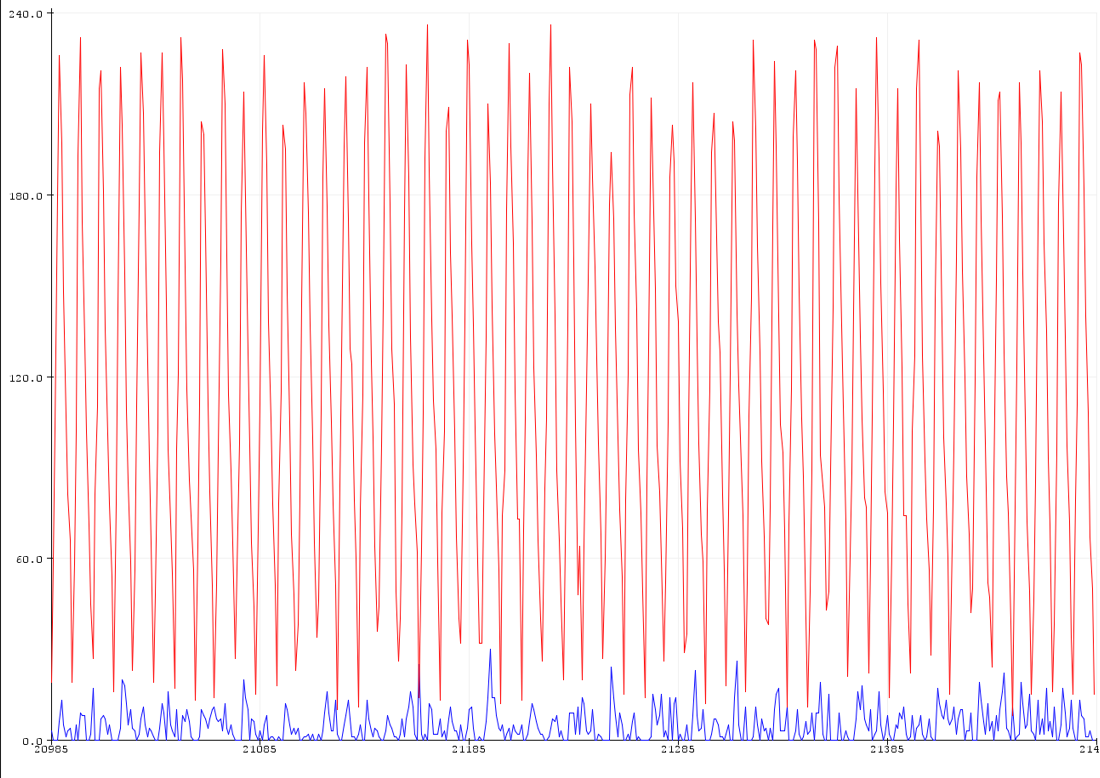
\includegraphics[width=\textwidth]{imaxes/resting.png}
      
    \end{subfigure}\\
    \caption{ActionButton}
  \end{tabular}    
 
\end{figure}

Como se puede ver a simple vista podemos apreciar una diferencia notable entre los 3 movimientos. La línea de plot azul se corresponde con el canal 1 y el músculo 




 %\chapter{Conclusións}
\label{chap:conclusions}

\lettrine{D}{erradeiro} capítulo da memoria, onde se presentará a
situación final do traballo, as leccións aprendidas, a relación coas
competencias da titulación en xeral e a mención en particular,
posibles liñas futuras,\dots

\Blindtext

 %\chapter{Contido demostrativo}
\label{chap:demo}

\lettrine{E}{ntre} a introdución e as conclusións, o documento conterá
tantos capítulos como sexa preciso, sempre con coidado de non rebasar
o límite de 80 páxinas fixado polo regulamento de TFGs.

Empregaremos éste de xeito demostrativo, para ilustrar o uso de
elementos habituais que poidan ser de utilidade\footnote{Por exemplo,
  isto é unha nota a pé de páxina.}.

\section{Inclusión de imaxes}

Se precisamos imaxes no noso documento, incluirémolas do xeito que se
indica na figura~\ref{fig:exemplo} (páxina~\pageref{fig:exemplo}). Se
o facemos así, \LaTeX ubicará cada imaxe no mellor lugar posible,
lugar que pode variar a medida que o documento vaia crecendo coa
inclusión de máis texto e outros elementos (máis imaxes, táboas,
etc.).

\begin{figure}[hp!]
  \centering
  
\includegraphics[width=0.75\textwidth]{imaxes/udc.png}
  \caption{Pé de imaxe descritivo}
  \label{fig:exemplo}
\end{figure}

Recoméndase almacenar os ficheiros gráficos no directorio
\texttt{imaxes}.

\subsection{Inclusión de varias sub-imaxes}

Se precisamos inserir imaxes relacionadas, pode ser apropiado
incluílas como sub-figuras, do xeito que se pode apreciar na
figura~\ref{fig:exemplo-subfiguras} coas
imaxes~\ref{fig:subfigura-rotada}
e~\ref{fig:subfigura-deformada}. Como se pode ver nos exemplos desta
sección, sempre é recomendable referirse ás imaxes pola súa
referencia, xa que dese xeito non dependemos de onde queden ubicados
os elementos en cuestión.

\begin{figure}[hp!]
  \centering
  \begin{subfigure}[c]{0.3\textwidth}
    
\includegraphics[angle=45,width=\textwidth]{imaxes/udc.png}
    \caption{Pé de subimaxe rotada}
    \label{fig:subfigura-rotada}
  \end{subfigure}
  \hspace{0.1\textwidth}
  \begin{subfigure}[c]{0.3\textwidth}
    
\includegraphics[width=\textwidth,height=3cm]{imaxes/udc.png}
    \caption{Pé de subimaxe deformada}
    \label{fig:subfigura-deformada}
  \end{subfigure}
  \caption{Pé de imaxe xeral}
  \label{fig:exemplo-subfiguras}
\end{figure}

\section{Inclusión de código fonte}

Se precisamos incluír fragmentos de código fonte, podemos facelo da
seguinte maneira:

\begin{lstlisting}[language=C]
#include <stdio.h>
#define N 10

int main()
{
  int i;

  // Isto é un comentario
  puts("Ola, mundo!");

  for (i = 0; i < N; i++)
  {
    puts("LaTeX é a ferramenta de edición ideal para profesionais da informática!");
  }

  return 0;
}
\end{lstlisting}

\section{Uso da relación de acrónimos e do glosario}

Os acrónimos edítanse no ficheiro \texttt{bibliografia/acronimos.tex}
e úsanse empregando a orde \texttt{acrlong} para obter o termo
completo (deste xeito: \acrlong{erlang}), a orde \texttt{acrshort}
para obter o acrónimo (deste xeito: \acrshort{erlang}). A primeira vez
que usamos un termo con acrónimo no documento é recomendable usar orde
\texttt{acrfull} (que produce ambas versións á vez:
\acrfull{erlang}). Os acrónimos que non se usan no documento, non
aparecen na relación que se xerar na versión PDF.

Pola súa banda, os termos do glosario edítanse no ficheiro
\texttt{bibliografia/glo\-sa\-rio.tex} e úsanse empregando a orde
\texttt{gls} (deste xeito, \gls{bytecode}) ou \texttt{Gls} (deste
xeito, \Gls{bytecode}). Ao igual que os acrónimos, os termos que non
se usan no documento, non aparecen na relación que se xera na versión
PDF.


 %%%%%%%%%%%%%%%%%%%%%%%%%%%%%%%%%%%%%%%%
 % Apéndices, glosarios e bibliografía  %
 %%%%%%%%%%%%%%%%%%%%%%%%%%%%%%%%%%%%%%%%

 %\appendix
 %\appendixpage
 %\chapter{Material adicional}
\label{chap:adicional}

\lettrine{E}{xemplo} de capítulo con formato de apéndice, onde se pode
incluír material adicional que non teña cabida no corpo principal do
documento, suxeito á limitación de 80 páxinas establecida no
regulamento de TFGs.

\Blindtext

 %\include{anexos/...}

 %\printglossary[type=\acronymtype,title=\nomeglosarioacronimos]
 %\printglossary[title=\nomeglosariotermos]

 \bibliographystyle{IEEEtranN}
 \bibliography{\bibconfig,bibliografia/bibliografia}
 \cleardoublepage
 
\end{document}

%%%%%%%%%%%%%%%%%%%%%%%%%%%%%%%%%%%%%%%%%%%%%%%%%%%%%%%%%%%%%%%%%%%%%%%%%%%%%%%%
